\documentclass[12pt,a4paper]{article}
\usepackage[utf8]{inputenc}
\usepackage[english]{babel}
\usepackage{geometry}
\geometry{a4paper, margin=2cm}
\usepackage{graphicx}
\usepackage{longtable}
\usepackage{hyperref}
\usepackage{array}
\usepackage{enumitem}
\usepackage{tabularx}
\usepackage{tikz}
\usetikzlibrary{fit, positioning, calc, arrows.meta, shapes.geometric}
\usepackage{pgfgantt}
\usepackage{microtype}
\usepackage{svg}
\usepackage[style=ieee,backend=biber]{biblatex}
\addbibresource{references.bib}

\begin{document}

% --- TRANG BÌA ---
\begin{titlepage}
    % Lệnh vẽ khung (border) cho trang bìa
    \begin{tikzpicture}[remember picture, overlay]
        \draw[line width = 2pt]
            ([shift={(1.5cm,-1.5cm)}]current page.north west)
            rectangle
            ([shift={(-1.5cm,1.5cm)}]current page.south east);
    \end{tikzpicture}
    
    \begin{center}
        \textbf{\large MINISTRY OF EDUCATION AND TRAINING} \\
        \vspace{0.2cm}
        \textbf{\large FPT UNIVERSITY} \\
        \textbf{---------------} \\
        \vspace{1cm}

        % Chèn Logo giả định
        \includesvg[width=0.4\textwidth]{Logo_Trường_Đại_học_FPT.svg} \\
        % \textit{[Logo FPT \& QS Stars Placeholder]} \\
        \vspace{2cm}
        
        \textbf{\Large MASTER OF SOFTWARE ENGINEERING (MSE)} \\
        \vspace{0.5cm}
        \textbf{\Large CAPSTONE PROJECT PROPOSAL} \\
        \vspace{2cm}

        \begin{flushleft}
            \textbf{\Large Project Title:} \\
            \vspace{0.5cm}
            \textbf{\LARGE IOT-BASED SMART CAMERA SYSTEM} \\
            \vspace{0.3cm}
            \textbf{\LARGE WITH FACE RECOGNITION AND} \\
            \vspace{0.3cm}
            \textbf{\LARGE ANOMALY DETECTION} \\
            \vspace{1cm}
        \end{flushleft}
        
        \begin{flushright}
            \textbf{Supervisor :} \textbf{Dr. Doan Xuan Huy Minh} \\
            \vspace{0.5cm}
            \textbf{Student :} \textbf{Nguyen Van Toan} \\
            \vspace{0.5cm}
            \textbf{Class :} \textbf{MSE26HCM}
        \end{flushright}
        
        \vfill
        HCM City, March 2026
    \end{center}
\end{titlepage}

\newpage

% --- MỤC LỤC ---
\tableofcontents
\newpage

% --- DANH MỤC TỪ VIẾT TẮT ---
\section*{LIST OF ABBREVIATIONS}
\addcontentsline{toc}{section}{LIST OF ABBREVIATIONS}

\begin{longtable}{|p{3cm}|p{12cm}|}
\hline
\textbf{Acronym} & \textbf{Full form} \\
\hline
\endhead
IoT & Internet of Things \\ \hline
AI & Artificial Intelligence \\ \hline
YOLO & You Only Look Once (Object Detection Model) \\ \hline
MSE & Master of Software Engineering \\ \hline
CV & Computer Vision \\ \hline
CPU & Central Processing Unit \\ \hline
API & Application Programming Interface \\ \hline
REST & Representational State Transfer \\ \hline
SMART & Specific, Measurable, Achievable, Relevant, and Time-bound \\ \hline
RQ & Research Question \\ \hline
TP./Tp. & City \\
\hline
\end{longtable}

\newpage
% --- PHẦN 1: DẪN NHẬP VÀ BỐI CẢNH ---
\section{Introduction and Background}
\subsection{Problem Description}
With the rapid development of smart home technologies, many households have adopted surveillance cameras to enhance security. However, most low-cost home camera systems only provide basic motion detection and video recording without intelligent identification or behavioral analysis capabilities.
Current commercial systems such as Google Nest Cam and Ring Video Doorbell offer advanced features including face recognition and cloud-based alerts. Nevertheless, these systems are relatively expensive, closed-source, and rely heavily on cloud services, raising concerns regarding privacy, customization, and long-term costs.
In many developing regions, families require a cost-effective and privacy-preserving solution that can:
\begin{itemize}
    \item Identify registered household members
    \item Detect unknown individuals
    \item Recognize abnormal entry behaviors
    \item Provide real-time alerts
\end{itemize}
There remains a research and practical gap in designing a lightweight, edge-based IoT camera system capable of real-time identification and anomaly detection suitable for small households \cite{sarimole_2024}. Addressing this issue is essential to enhance home security, reduce burglary risks, and promote affordable smart home adoption \cite{ijacsa_2020}.

\subsection{Research Objectives}
The project aims to develop an IoT-based smart camera system with the following SMART objectives:
\begin{itemize}
    \item Develop a real-time face recognition system achieving at least 90\% identification accuracy under controlled indoor conditions.
    \item Implement an anomaly detection mechanism capable of detecting unknown individuals and entry at unusual hours \cite{facenet_2015}.
    \item Ensure system response time is less than 5 seconds from detection to notification \cite{gupta_edge_2020}.
    \item Deliver a fully functional prototype within 14 weeks.
\end{itemize}

\subsubsection{Literature Review and Gap Analysis}
To address the research questions, a comparison of existing solutions and the proposed system is presented in Table \ref{tab:comparison}.

\begin{table}[h]
    \centering
    \caption{Comparison of Existing Solutions vs. Proposed Smart Camera}
    \label{tab:comparison}
    \begin{tabular}{|l|c|c|c|c|}
        \hline
        \textbf{Feature} & \textbf{Nest Cam} & \textbf{Ring Doorbell} & \textbf{OpenCV/Pi} & \textbf{Proposed System} \\ \hline
        Face Recognition & Advanced & Cloud-based & Basic & Advanced (FaceNet) \\ \hline
        Privacy & Cloud-only & Cloud-only & Local & Local (Edge AI) \\ \hline
        Anomaly Detection & Limited & Limited & Manual & Automated (YOLOv8) \\ \hline
        Cost & High & High & Low & Low-Moderate \\ \hline
        Connectivity & Constant & Constant & Offline/Local & Hybrid \\ \hline
    \end{tabular}
\end{table}

\subsubsection{Research Questions}
\begin{itemize}
    \item \textit{RQ1:} What existing face recognition and anomaly detection methods can solve this problem? What are their advantages and disadvantages?
    \item \textit{RQ2:} What method and architecture will be proposed in this project? How will it be implemented on an IoT edge device?
    \item \textit{RQ3:} How will the performance, accuracy, and usability of the system be evaluated?
\end{itemize}

\subsection{Scope of the Project}
\textbf{Included:}
\begin{itemize}
    \item Face registration of household members and real-time face recognition.
    \item Unknown person detection and rule-based anomaly detection.
    \item Web dashboard for monitoring and notification system (email or app).
\end{itemize}
\textbf{Excluded:}
\begin{itemize}
    \item Full smart home integration and large-scale cloud deployment.
    \item Emotion recognition and complex behavioral AI analysis.
\end{itemize}

% --- PHẦN 2: GIẢI PHÁP ĐỀ XUẤT ---
\section{Proposed Solution}
\subsection{Solution Description}
The proposed system is an IoT-based smart camera solution integrating edge AI processing and backend services \cite{sarimole_2024}. The system processes video streams locally (edge computing) to reduce latency and preserve privacy \cite{sahu_2023}. Recognition results are transmitted to the backend server for logging and notification, with an emphasis on a user-friendly interface for residents \cite{ux_iot_2024}.

\subsection{Software Architecture (General)}
The system adopts a Client-Server architecture with Edge AI processing, as illustrated in Figure \ref{fig:architecture}.

\begin{figure}[h]
    \centering
    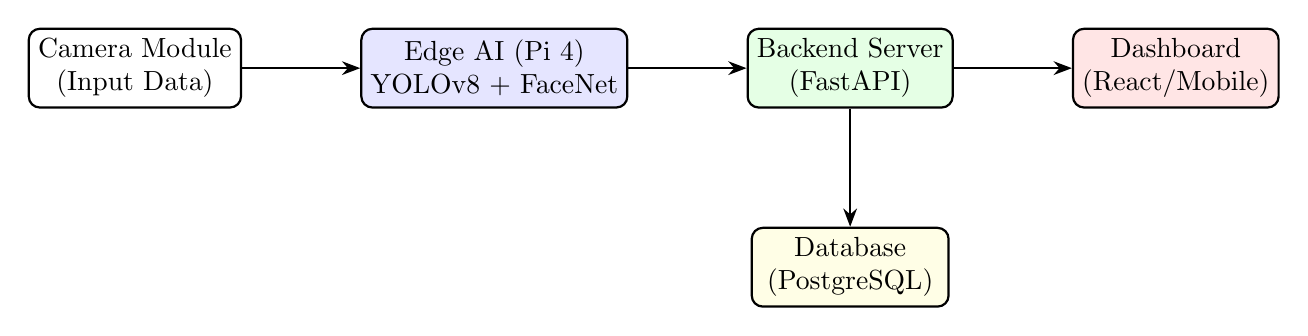
\begin{tikzpicture}[
        node distance=1.5cm,
        box/.style={rectangle, draw=black, thick, minimum width=2.5cm, minimum height=1cm, align=center, rounded corners},
        arrow/.style={-Stealth, thick}
    ]
        % Nodes
        \node[box] (camera) {Camera Module\\(Input Data)};
        \node[box, right=of camera, fill=blue!10] (edge) {Edge AI (Pi 4)\\{YOLOv8 + FaceNet}};
        \node[box, right=of edge, fill=green!10] (backend) {Backend Server\\(FastAPI)};
        \node[box, below=of backend, fill=yellow!10] (db) {Database\\(PostgreSQL)};
        \node[box, right=of backend, fill=red!10] (frontend) {Dashboard\\(React/Mobile)};

        % Connectors
        \draw[arrow] (camera) -- (edge);
        \draw[arrow] (edge) -- (backend);
        \draw[arrow] (backend) -- (db);
        \draw[arrow] (backend) -- (frontend);
    \end{tikzpicture}
    \caption{System Architecture Diagram}
    \label{fig:architecture}
\end{figure}

\begin{itemize}
    \item \textbf{Edge Layer:} Face detection using YOLOv8 \cite{yolov8_2023}; Face recognition using FaceNet embeddings.
    \item \textbf{Backend Layer:} REST API using FastAPI \cite{fastapi_2020}; PostgreSQL database for logging.
    \item \textbf{Frontend Layer:} ReactJS/NextJS dashboard for monitoring alerts.
\end{itemize}

\subsection{Technology and Tools Used}
\begin{itemize}
    \item \textbf{Hardware:} Raspberry Pi 4 Model B (8GB RAM), Raspberry Pi Camera Module V2 (8MP).
    \item \textbf{AI \& Computer Vision:} Python 3.10, OpenCV 4.8, FaceNet (Keras-based), YOLOv8.
    \item \textbf{Backend:} FastAPI, PostgreSQL, SQLAlchemy.
    \item \textbf{Frontend:} Next.js, React Native (for mobile alerts).
\end{itemize}

% --- PHẦN 3: KẾ HOẠCH TRIỂN KHAI ---
\section{Implementation Plan}
\subsection{Main Development Stages}
\begin{enumerate}
    \item Phase 1 – Requirements Analysis
    \item Phase 2 – Literature Review and Model Comparison
    \item Phase 3 – System Design
    \item Phase 4 – Development and Integration
    \item Phase 5 – Testing and Optimization
    \item Phase 6 – Final Deployment and Documentation
\end{enumerate}

\subsection{Expected Schedule (Preliminary)}
\begin{table}[h]
    \centering
    \caption{Preliminary Project Schedule}
    \begin{tabular}{|l|l|}
        \hline
        \textbf{Timeframes} & \textbf{Activities} \\ \hline
        Weeks 1--2 & Requirement Analysis and Research \\ \hline
        Weeks 3--4 & Model Evaluation and Architecture Design \\ \hline
        Weeks 5--8 & Core System Development \\ \hline
        Weeks 9--11 & Integration and Dashboard Development \\ \hline
        Weeks 12--13 & Testing and Performance Evaluation \\ \hline
        Week 14 & Final Report and Presentation \\ \hline
    \end{tabular}
\end{table}

\subsection{Feasibility Assessment}
\begin{itemize}
    \item \textbf{Technical Challenges:} Low-light recognition accuracy, edge device computational limitations (CPU/RAM).
    \item \textbf{Mitigation:} Image preprocessing (normalization), lightweight models (YOLOv8-Nano), and multi-threading.
    \item \textbf{Resources:} Raspberry Pi 4, Sony IMX219 sensor, Labeled Faces in the Wild (LFW) dataset for pre-training, and locally captured dataset (family faces) for fine-tuning.
\end{itemize}

% --- PHẦN 4 & 5: KẾT QUẢ VÀ ĐÁNH GIÁ ---
\section{Expected Results}
Upon completion, the project will deliver:
\begin{itemize}
    \item A fully functional IoT smart camera prototype.
    \item Face recognition accuracy $\ge$ 85\%.
    \item Alert response time $\le$ 5 seconds.
    \item Web dashboard for monitoring and source code documentation.
\end{itemize}

\section{Evaluation Plan}
The system will be evaluated using:
\begin{itemize}
    \item \textbf{Technical Metrics:} Accuracy, Precision, Recall, F1-score, Confusion Matrix \cite{ijacsa_2020}.
    \item \textbf{Performance Metrics:} Detection Latency (ms), Identification Latency (ms), CPU/RAM usage \cite{sarimole_2024}.
    \item \textbf{Network Metrics:} Data throughput under Wi-Fi, 4G, and limited connectivity scenarios.
    \item \textbf{User Evaluation:} Usability testing (System Usability Scale) and user satisfaction survey targeting UI/UX efficiency \cite{haney_2025}.
\end{itemize}

% --- PHẦN 6: TÀI LIỆU THAM KHẢO ---
\section{References}
% Tất cả tài liệu phải được trích dẫn theo chuẩn IEEE [6, 21].
% Sử dụng biblatex để tự động hóa phần này.

\printbibliography
\end{document}